\section{Overview}
\label{sec:buffer-control}
RxJava points out on its wiki page about backpressure \cite{RxJava-Wiki-Backpressure} that it does not make the problem of overproduction in the source go away. It claims to only move ``\textit{the problem up the chain of operators to a point where it can be handled better}''. To do so, they created the \textit{reactive pull} mechanism with operators like \code{onBackpressureBuffer} and \code{onBackpressureDrop}, such that the flow control is moved up to these kinds of operators.

We propose to move this flow control even further up the chain; up to the point where the source of the stream is drained in the pipeline of operators. Only there we can have maximum control over how much data is brought into the stream at a particular point in time. With this we do not have the need for infinite buffers as is the case in \code{onBackpressureBuffer}, nor do we have to drop unprocessed elements as is done with \code{onBackpressureDrop}. We propose to not wrap the cold source in the \code{Observable.create} (or any of its derived factory methods) but to wrap it in a universal, interactive interface. This way we are not dependent in our implementation on what kind of source we are dealing with. Given this interactive interface we can fill a \textit{bounded} buffer with as many elements as can be processed at a particular point in time. The buffer pulls data from the source on behalf of the subscriber, which gets as much data pushed at it as it is able to handle. Pushing an element from the buffer to the downstream will automatically block the thread for another element to be pushed until the first one is fully processed.

Since we want to control the buffer's size, we have to observe that control over how many elements will flow into the buffer is to a certain extends in our own hands. However, how fast the downstream is going to drain the buffer is an unknown fact. Therefore we will use feedback control to respond to the uncertainty that the downstream brings in. It does, however, not make sense to give a certain fixed size to the setpoint and compare the current size with it. After all, some `slow' consumer might go faster or slower than expected. Controlling the buffer with a certain fixed size defeats the purpose of the feedback system in this case, as we cannot dynamically grow or shrink the size as needed. On the other hand, it is also not possible to ask ``\textit{make sure the buffer is filled to its optimal size}''. A feedback system is not able to solve this, as this does not have a particular setpoint specified \cite{janert2013-feedback}.

Instead of controlling the buffer size directly, we choose to measure the ratio between what goes out the buffer and what comes in the buffer. We will refer to this ratio as the system's throughput. In an optimal situation the amount of data that comes in is just as much as comes out of the system, so ideally this ratio must be $1.0$, which will be the setpoint of this system. Given the error that comes from the difference between the setpoint and the actual throughput, we can then determine how many elements to request from the source in the next iteration. The controller that does this will be discussed in a later section.

The full feedback system is depicted in \Cref{fig:backpressure-feedback-system}. In this figure the \textit{SRC control} receives a number \code{n} of elements to be requested from source \textit{SRC}. Eventually these elements get delivered and are stored in the buffer inside \textit{Buffer control}. The \textit{Downstream handler} pulls elements from the buffer and sends them downstream to be processed further in the reactive operator sequence. \textit{Buffer control} measures the throughput $\tau$ and sends this to the setpoint \code{sp} to be compared with. The resulting error \code{e} is then transformed into a new \code{n} inside an incremental controller \textit{C} and an integrator $\Sigma$.

\begin{figure}[H]
	\begin{center}
		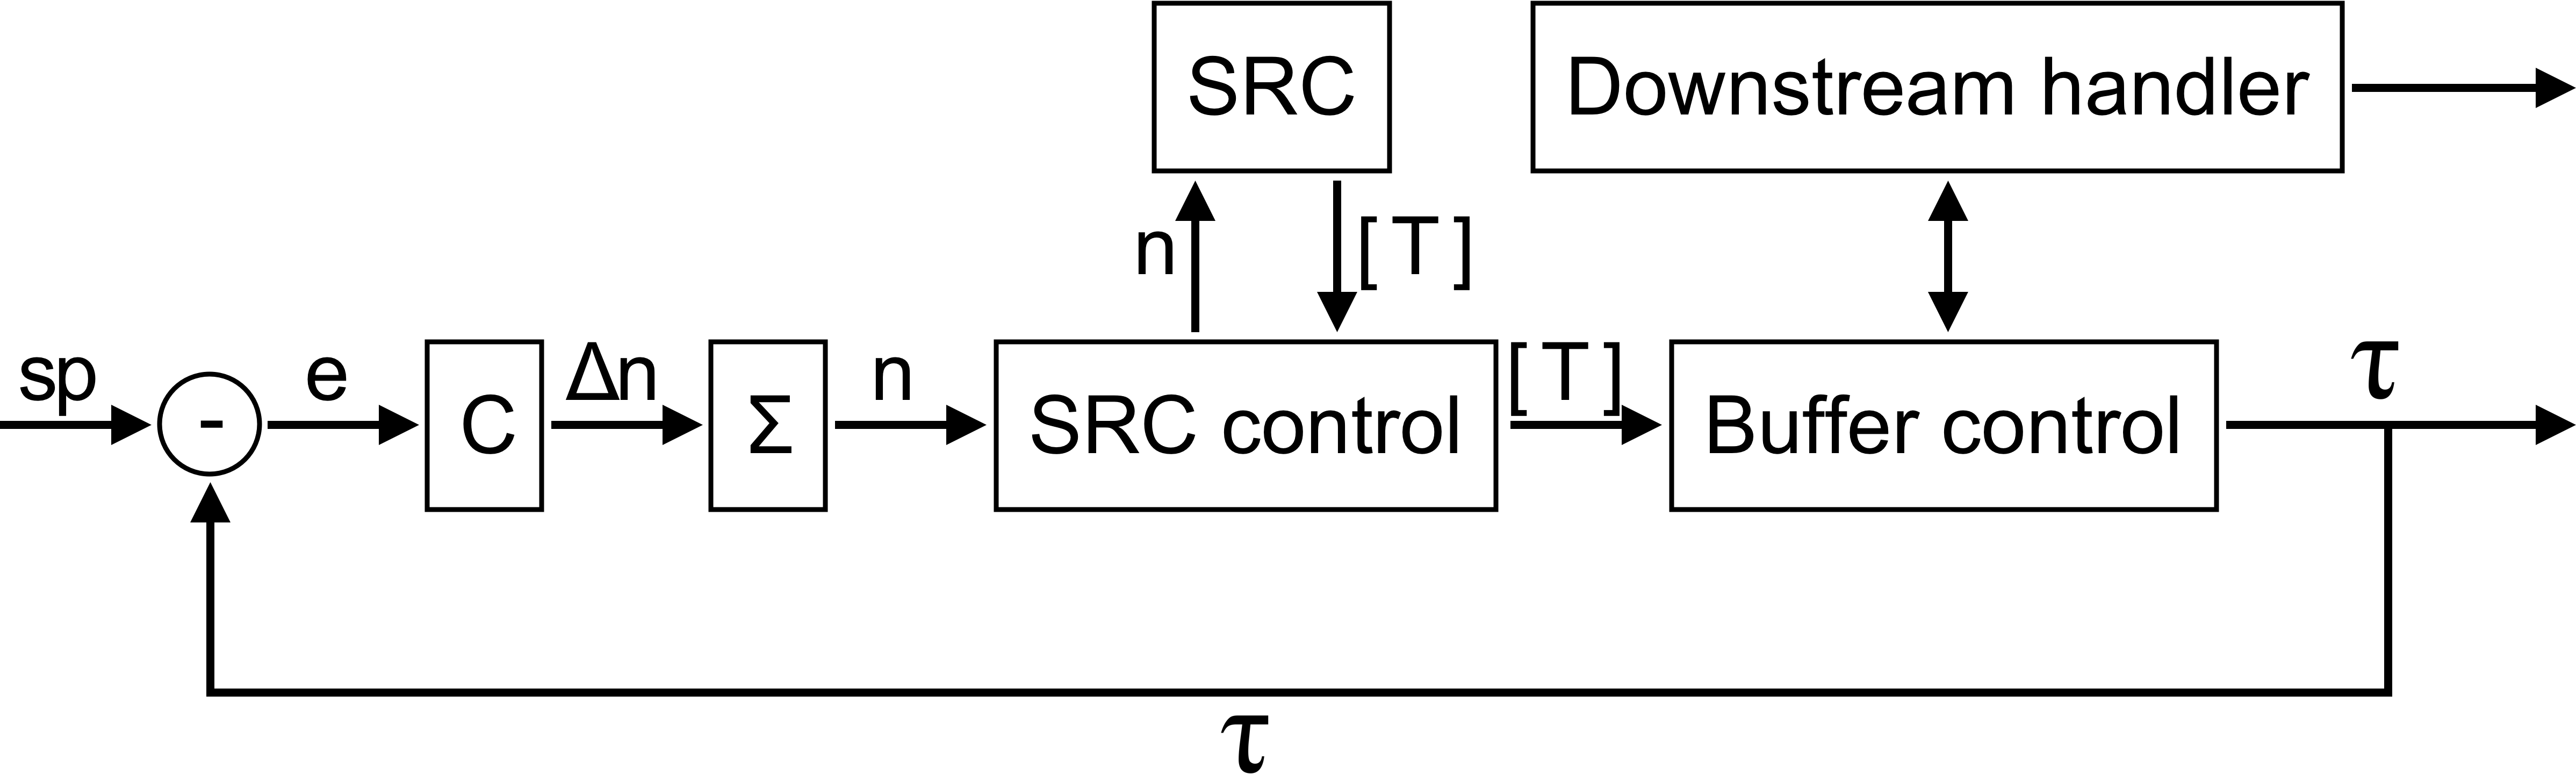
\includegraphics[width=0.8\textwidth]{figures/Backpressure-feedback-system.png}
	\end{center}
	\caption{Feedback system for controlling overproduction}
	\label{fig:backpressure-feedback-system}
\end{figure}

It becomes clear from this figure that the source itself is not part of the feedback system, but is instead used by the system to retrieve a certain number of elements from. Also note that the \textit{downstream handler} is not part of feedback system either. Even though it \emph{interacts} with the buffer, it is an external force that influences the behavior of the system. Ultimately the \textit{Downstream handler} is the part that exposes an \obs for an \obv to listen to.

Compared to Reactive Streams and RxJava's reactive pull implementation, our approach has the major advantage of keeping the overflow protection to the only place it can be controlled from: the source of the stream. This allows us to keep the set of operators defined on the reactive interface clean and only have the responsibility of applying a specific functionality to the events that come in. Contrast this with RxJava's backpressure implementation where every operator has to also deal with the question of how many elements it is willing to receive next. This is equal to having our solution of controlling overproduction in every single operator.
